% Generated by Sphinx.
\def\sphinxdocclass{report}
\documentclass[letterpaper,10pt,openany,oneside]{sphinxmanual}
\usepackage[utf8]{inputenc}
\DeclareUnicodeCharacter{00A0}{\nobreakspace}
\usepackage[T1]{fontenc}
\usepackage[english]{babel}
\usepackage{times}
\usepackage[Bjarne]{fncychap}
\usepackage{longtable}
\usepackage{sphinx}
\usepackage{multirow}
\usepackage{booktabs}
\usepackage{array}
\definecolor{nrelblue}{RGB}{0, 121, 193}
\hypersetup{linkcolor=nrelblue}
\usepackage[section]{placeins}


\title{turbine_costSE Documentation}
\date{August 30, 2013}
\release{0.1.0}
\author{Katherine Dykes}
\newcommand{\sphinxlogo}{}
\renewcommand{\releasename}{Release}
\makeindex

\makeatletter
\def\PYG@reset{\let\PYG@it=\relax \let\PYG@bf=\relax%
    \let\PYG@ul=\relax \let\PYG@tc=\relax%
    \let\PYG@bc=\relax \let\PYG@ff=\relax}
\def\PYG@tok#1{\csname PYG@tok@#1\endcsname}
\def\PYG@toks#1+{\ifx\relax#1\empty\else%
    \PYG@tok{#1}\expandafter\PYG@toks\fi}
\def\PYG@do#1{\PYG@bc{\PYG@tc{\PYG@ul{%
    \PYG@it{\PYG@bf{\PYG@ff{#1}}}}}}}
\def\PYG#1#2{\PYG@reset\PYG@toks#1+\relax+\PYG@do{#2}}

\expandafter\def\csname PYG@tok@gd\endcsname{\def\PYG@tc##1{\textcolor[rgb]{0.63,0.00,0.00}{##1}}}
\expandafter\def\csname PYG@tok@gu\endcsname{\let\PYG@bf=\textbf\def\PYG@tc##1{\textcolor[rgb]{0.50,0.00,0.50}{##1}}}
\expandafter\def\csname PYG@tok@gt\endcsname{\def\PYG@tc##1{\textcolor[rgb]{0.00,0.25,0.82}{##1}}}
\expandafter\def\csname PYG@tok@gs\endcsname{\let\PYG@bf=\textbf}
\expandafter\def\csname PYG@tok@gr\endcsname{\def\PYG@tc##1{\textcolor[rgb]{1.00,0.00,0.00}{##1}}}
\expandafter\def\csname PYG@tok@cm\endcsname{\let\PYG@it=\textit\def\PYG@tc##1{\textcolor[rgb]{0.25,0.50,0.56}{##1}}}
\expandafter\def\csname PYG@tok@vg\endcsname{\def\PYG@tc##1{\textcolor[rgb]{0.73,0.38,0.84}{##1}}}
\expandafter\def\csname PYG@tok@m\endcsname{\def\PYG@tc##1{\textcolor[rgb]{0.13,0.50,0.31}{##1}}}
\expandafter\def\csname PYG@tok@mh\endcsname{\def\PYG@tc##1{\textcolor[rgb]{0.13,0.50,0.31}{##1}}}
\expandafter\def\csname PYG@tok@cs\endcsname{\def\PYG@tc##1{\textcolor[rgb]{0.25,0.50,0.56}{##1}}\def\PYG@bc##1{\setlength{\fboxsep}{0pt}\colorbox[rgb]{1.00,0.94,0.94}{\strut ##1}}}
\expandafter\def\csname PYG@tok@ge\endcsname{\let\PYG@it=\textit}
\expandafter\def\csname PYG@tok@vc\endcsname{\def\PYG@tc##1{\textcolor[rgb]{0.73,0.38,0.84}{##1}}}
\expandafter\def\csname PYG@tok@il\endcsname{\def\PYG@tc##1{\textcolor[rgb]{0.13,0.50,0.31}{##1}}}
\expandafter\def\csname PYG@tok@go\endcsname{\def\PYG@tc##1{\textcolor[rgb]{0.19,0.19,0.19}{##1}}}
\expandafter\def\csname PYG@tok@cp\endcsname{\def\PYG@tc##1{\textcolor[rgb]{0.00,0.44,0.13}{##1}}}
\expandafter\def\csname PYG@tok@gi\endcsname{\def\PYG@tc##1{\textcolor[rgb]{0.00,0.63,0.00}{##1}}}
\expandafter\def\csname PYG@tok@gh\endcsname{\let\PYG@bf=\textbf\def\PYG@tc##1{\textcolor[rgb]{0.00,0.00,0.50}{##1}}}
\expandafter\def\csname PYG@tok@ni\endcsname{\let\PYG@bf=\textbf\def\PYG@tc##1{\textcolor[rgb]{0.84,0.33,0.22}{##1}}}
\expandafter\def\csname PYG@tok@nl\endcsname{\let\PYG@bf=\textbf\def\PYG@tc##1{\textcolor[rgb]{0.00,0.13,0.44}{##1}}}
\expandafter\def\csname PYG@tok@nn\endcsname{\let\PYG@bf=\textbf\def\PYG@tc##1{\textcolor[rgb]{0.05,0.52,0.71}{##1}}}
\expandafter\def\csname PYG@tok@no\endcsname{\def\PYG@tc##1{\textcolor[rgb]{0.38,0.68,0.84}{##1}}}
\expandafter\def\csname PYG@tok@na\endcsname{\def\PYG@tc##1{\textcolor[rgb]{0.25,0.44,0.63}{##1}}}
\expandafter\def\csname PYG@tok@nb\endcsname{\def\PYG@tc##1{\textcolor[rgb]{0.00,0.44,0.13}{##1}}}
\expandafter\def\csname PYG@tok@nc\endcsname{\let\PYG@bf=\textbf\def\PYG@tc##1{\textcolor[rgb]{0.05,0.52,0.71}{##1}}}
\expandafter\def\csname PYG@tok@nd\endcsname{\let\PYG@bf=\textbf\def\PYG@tc##1{\textcolor[rgb]{0.33,0.33,0.33}{##1}}}
\expandafter\def\csname PYG@tok@ne\endcsname{\def\PYG@tc##1{\textcolor[rgb]{0.00,0.44,0.13}{##1}}}
\expandafter\def\csname PYG@tok@nf\endcsname{\def\PYG@tc##1{\textcolor[rgb]{0.02,0.16,0.49}{##1}}}
\expandafter\def\csname PYG@tok@si\endcsname{\let\PYG@it=\textit\def\PYG@tc##1{\textcolor[rgb]{0.44,0.63,0.82}{##1}}}
\expandafter\def\csname PYG@tok@s2\endcsname{\def\PYG@tc##1{\textcolor[rgb]{0.25,0.44,0.63}{##1}}}
\expandafter\def\csname PYG@tok@vi\endcsname{\def\PYG@tc##1{\textcolor[rgb]{0.73,0.38,0.84}{##1}}}
\expandafter\def\csname PYG@tok@nt\endcsname{\let\PYG@bf=\textbf\def\PYG@tc##1{\textcolor[rgb]{0.02,0.16,0.45}{##1}}}
\expandafter\def\csname PYG@tok@nv\endcsname{\def\PYG@tc##1{\textcolor[rgb]{0.73,0.38,0.84}{##1}}}
\expandafter\def\csname PYG@tok@s1\endcsname{\def\PYG@tc##1{\textcolor[rgb]{0.25,0.44,0.63}{##1}}}
\expandafter\def\csname PYG@tok@gp\endcsname{\let\PYG@bf=\textbf\def\PYG@tc##1{\textcolor[rgb]{0.78,0.36,0.04}{##1}}}
\expandafter\def\csname PYG@tok@sh\endcsname{\def\PYG@tc##1{\textcolor[rgb]{0.25,0.44,0.63}{##1}}}
\expandafter\def\csname PYG@tok@ow\endcsname{\let\PYG@bf=\textbf\def\PYG@tc##1{\textcolor[rgb]{0.00,0.44,0.13}{##1}}}
\expandafter\def\csname PYG@tok@sx\endcsname{\def\PYG@tc##1{\textcolor[rgb]{0.78,0.36,0.04}{##1}}}
\expandafter\def\csname PYG@tok@bp\endcsname{\def\PYG@tc##1{\textcolor[rgb]{0.00,0.44,0.13}{##1}}}
\expandafter\def\csname PYG@tok@c1\endcsname{\let\PYG@it=\textit\def\PYG@tc##1{\textcolor[rgb]{0.25,0.50,0.56}{##1}}}
\expandafter\def\csname PYG@tok@kc\endcsname{\let\PYG@bf=\textbf\def\PYG@tc##1{\textcolor[rgb]{0.00,0.44,0.13}{##1}}}
\expandafter\def\csname PYG@tok@c\endcsname{\let\PYG@it=\textit\def\PYG@tc##1{\textcolor[rgb]{0.25,0.50,0.56}{##1}}}
\expandafter\def\csname PYG@tok@mf\endcsname{\def\PYG@tc##1{\textcolor[rgb]{0.13,0.50,0.31}{##1}}}
\expandafter\def\csname PYG@tok@err\endcsname{\def\PYG@bc##1{\setlength{\fboxsep}{0pt}\fcolorbox[rgb]{1.00,0.00,0.00}{1,1,1}{\strut ##1}}}
\expandafter\def\csname PYG@tok@kd\endcsname{\let\PYG@bf=\textbf\def\PYG@tc##1{\textcolor[rgb]{0.00,0.44,0.13}{##1}}}
\expandafter\def\csname PYG@tok@ss\endcsname{\def\PYG@tc##1{\textcolor[rgb]{0.32,0.47,0.09}{##1}}}
\expandafter\def\csname PYG@tok@sr\endcsname{\def\PYG@tc##1{\textcolor[rgb]{0.14,0.33,0.53}{##1}}}
\expandafter\def\csname PYG@tok@mo\endcsname{\def\PYG@tc##1{\textcolor[rgb]{0.13,0.50,0.31}{##1}}}
\expandafter\def\csname PYG@tok@mi\endcsname{\def\PYG@tc##1{\textcolor[rgb]{0.13,0.50,0.31}{##1}}}
\expandafter\def\csname PYG@tok@kn\endcsname{\let\PYG@bf=\textbf\def\PYG@tc##1{\textcolor[rgb]{0.00,0.44,0.13}{##1}}}
\expandafter\def\csname PYG@tok@o\endcsname{\def\PYG@tc##1{\textcolor[rgb]{0.40,0.40,0.40}{##1}}}
\expandafter\def\csname PYG@tok@kr\endcsname{\let\PYG@bf=\textbf\def\PYG@tc##1{\textcolor[rgb]{0.00,0.44,0.13}{##1}}}
\expandafter\def\csname PYG@tok@s\endcsname{\def\PYG@tc##1{\textcolor[rgb]{0.25,0.44,0.63}{##1}}}
\expandafter\def\csname PYG@tok@kp\endcsname{\def\PYG@tc##1{\textcolor[rgb]{0.00,0.44,0.13}{##1}}}
\expandafter\def\csname PYG@tok@w\endcsname{\def\PYG@tc##1{\textcolor[rgb]{0.73,0.73,0.73}{##1}}}
\expandafter\def\csname PYG@tok@kt\endcsname{\def\PYG@tc##1{\textcolor[rgb]{0.56,0.13,0.00}{##1}}}
\expandafter\def\csname PYG@tok@sc\endcsname{\def\PYG@tc##1{\textcolor[rgb]{0.25,0.44,0.63}{##1}}}
\expandafter\def\csname PYG@tok@sb\endcsname{\def\PYG@tc##1{\textcolor[rgb]{0.25,0.44,0.63}{##1}}}
\expandafter\def\csname PYG@tok@k\endcsname{\let\PYG@bf=\textbf\def\PYG@tc##1{\textcolor[rgb]{0.00,0.44,0.13}{##1}}}
\expandafter\def\csname PYG@tok@se\endcsname{\let\PYG@bf=\textbf\def\PYG@tc##1{\textcolor[rgb]{0.25,0.44,0.63}{##1}}}
\expandafter\def\csname PYG@tok@sd\endcsname{\let\PYG@it=\textit\def\PYG@tc##1{\textcolor[rgb]{0.25,0.44,0.63}{##1}}}

\def\PYGZbs{\char`\\}
\def\PYGZus{\char`\_}
\def\PYGZob{\char`\{}
\def\PYGZcb{\char`\}}
\def\PYGZca{\char`\^}
\def\PYGZam{\char`\&}
\def\PYGZlt{\char`\<}
\def\PYGZgt{\char`\>}
\def\PYGZsh{\char`\#}
\def\PYGZpc{\char`\%}
\def\PYGZdl{\char`\$}
\def\PYGZti{\char`\~}
% for compatibility with earlier versions
\def\PYGZat{@}
\def\PYGZlb{[}
\def\PYGZrb{]}
\makeatother

\begin{document}

%\maketitle
%\tableofcontents
%\phantomsection\label{index::doc}



\chapter{Introduction}
\label{intro:introduction}\label{intro::doc}\label{intro:turbine-costse}
The set of models contained in this software allow for the determination of costs for major hub and drivetrain components of a wind turbine based on their masses and a few other select parameters.  The software combines sources of information from several areas: The NREL Cost and Scaling Model {\hyperref[theory:1]{{[}1{]}}} and related subsequent cost model development efforts, the Wind Partnerships for Advanced Component Technology (WindPACT) work that occurred between roughly 2002 to 2005 {\hyperref[theory:2]{{[}2{]}}}, and the University of Sunderland (the Sunderland Model) {\hyperref[theory:3]{{[}3{]}}}.  These mass-cost models use the data from the sources above to take the component mass and estimate the associated cost in a reference year and month.  The component cost can then be scaled to a different year and month based on economic multipliers as done in {\hyperref[theory:1]{{[}1{]}}}.


\chapter{Installation}
\label{installation:installation}\label{installation::doc}
\begin{notice}{note}{prerequisites}

NumPy, SciPy
\end{notice}

Download either masstocost.py-0.1.0.tar.gz or masstocost.py-0.1.0.zip, and uncompress/unpack it.

Install HubNacelleCST with the following command.

\begin{quote}
\begin{Verbatim}[commandchars=\\\{\}]
\PYG{n+nv}{\PYGZdl{} }python setup.py install
\end{Verbatim}
\end{quote}

To check if installation was successful run the unit tests for the NREL 5MW model

\begin{quote}
\begin{Verbatim}[commandchars=\\\{\}]
\PYG{n+nv}{\PYGZdl{} }python \PYG{n+nb}{test}/test\PYGZus{}masstocost.py
\end{Verbatim}
\end{quote}

An `OK' signifies that all the tests passed.

To access an HTML version of this documentation which contains further details and links to the source code, open docs/index.html.


\chapter{Tutorial}
\label{tutorial:tutorial-label}\label{tutorial::doc}\label{tutorial:tutorial}
As an example, let us simulate using masses for major wind turbine components for the NREL 5MW Reference Model {[}Jonkman2009{]} using the overall turbine cost model.  The hub and drivetrain component masses must also be provided and are calculated from Sunderland Model {\hyperref[theory:3]{{[}3{]}}}.

The first step is to import the relevant files and set up the PPI indices based on the years of interest (reference and current).

\begin{quote}
\begin{Verbatim}[commandchars=\\\{\}]
\PYG{k+kn}{from} \PYG{n+nn}{turbine\PYGZus{}costSE.src.turbine\PYGZus{}costSE} \PYG{k+kn}{import} \PYG{n}{TurbineCost}
\PYG{k+kn}{from} \PYG{n+nn}{turbine\PYGZus{}costSE.src.config} \PYG{k+kn}{import} \PYG{o}{*}

\PYG{c}{\PYGZsh{} simple example of the turbine cost model}

\PYG{n}{ref\PYGZus{}yr}  \PYG{o}{=} \PYG{l+m+mi}{2002}
\PYG{n}{ref\PYGZus{}mon} \PYG{o}{=}    \PYG{l+m+mi}{9}
\PYG{n}{curr\PYGZus{}yr} \PYG{o}{=} \PYG{l+m+mi}{2009}
\PYG{n}{curr\PYGZus{}mon} \PYG{o}{=}  \PYG{l+m+mi}{12}

\PYG{n}{ppi}\PYG{o}{.}\PYG{n}{ref\PYGZus{}yr}   \PYG{o}{=} \PYG{n}{ref\PYGZus{}yr}
\PYG{n}{ppi}\PYG{o}{.}\PYG{n}{ref\PYGZus{}mon}  \PYG{o}{=} \PYG{n}{ref\PYGZus{}mon}
\end{Verbatim}
\end{quote}

The turbine cost model relies on the mass inputs of all major turbine components.  These filter down to the individual component models through the rotor, nacelle and tower.

\begin{quote}
\begin{Verbatim}[commandchars=\\\{\}]
\PYG{c}{\PYGZsh{} NREL 5 MW turbine component masses based on Sunderland model approach}
\PYG{n}{bladeMass} \PYG{o}{=} \PYG{l+m+mf}{17650.67}  
\PYG{n}{hubMass} \PYG{o}{=} \PYG{l+m+mf}{31644.5}
\PYG{n}{pitchSystemMass} \PYG{o}{=} \PYG{l+m+mf}{17004.0}
\PYG{n}{spinnerMass} \PYG{o}{=} \PYG{l+m+mf}{1810.5}

\PYG{n}{lssMass} \PYG{o}{=} \PYG{l+m+mf}{31257.3}
\PYG{n}{bearingsMass} \PYG{o}{=} \PYG{l+m+mf}{9731.41}
\PYG{n}{gearboxMass} \PYG{o}{=} \PYG{l+m+mf}{30237.60}
\PYG{n}{hssMass} \PYG{o}{=} \PYG{l+m+mf}{1492.45}
\PYG{n}{generatorMass} \PYG{o}{=} \PYG{l+m+mf}{16699.85}
\PYG{n}{bedplateMass} \PYG{o}{=} \PYG{l+m+mf}{93090.6}
\PYG{n}{yawSystemMass} \PYG{o}{=} \PYG{l+m+mf}{11878.24}

\PYG{n}{towerMass} \PYG{o}{=} \PYG{l+m+mf}{434559.0}
\end{Verbatim}
\end{quote}

Next, we need to set additional inputs to the model.  The blade number must be known to get the total cost for the blade set; the advanced Boolean for the blade must be set to select which mass-cost curve for the blade to use (normal or advanced blade).  We set this to advanced to be in line with the FAST 5 MW reference model.  The machine rating and boolean flags for onboard crane and offshore project must also be set.  These are used in the determination of costs for auxiliary system components.  Finally, the drivetrain configuration (iDesign) is specified so that the proper gearbox and generator coefficients will be used.  This should always be set to 1 for the current model.

\begin{quote}
\begin{Verbatim}[commandchars=\\\{\}]
\PYG{c}{\PYGZsh{} Additional non-mass cost model input variables}
\PYG{n}{bladeNum} \PYG{o}{=} \PYG{l+m+mi}{3}
\PYG{n}{advanced} \PYG{o}{=} \PYG{n+nb+bp}{True} \PYG{c}{\PYGZsh{} use advanced blade mass-cost curve}
\PYG{n}{machineRating} \PYG{o}{=} \PYG{l+m+mf}{5000.0}
\PYG{n}{iDesign} \PYG{o}{=} \PYG{l+m+mi}{1} \PYG{c}{\PYGZsh{} conventional 3-stage geared drivetrain system}
\PYG{n}{crane} \PYG{o}{=} \PYG{n+nb+bp}{True} \PYG{c}{\PYGZsh{} onboard crane is present}
\PYG{n}{offshore} \PYG{o}{=} \PYG{n+nb+bp}{True} \PYG{c}{\PYGZsh{} turbine is for an offshore application}
\end{Verbatim}
\end{quote}

We can now create and evaluate the cost for the turbine and its components.

\begin{quote}
\begin{Verbatim}[commandchars=\\\{\}]
\PYG{n}{turbine} \PYG{o}{=} \PYG{n}{TurbineCost}\PYG{p}{(}\PYG{n}{bladeMass}\PYG{p}{,} \PYG{n}{bladeNum}\PYG{p}{,} \PYG{n}{hubMass}\PYG{p}{,} \PYG{n}{pitchSystemMass}\PYG{p}{,} \PYG{n}{spinnerMass}\PYG{p}{,} \PYG{n}{towerMass}\PYG{p}{,} \PYG{n}{lssMass}\PYG{p}{,} \PYGZbs{}
                     \PYG{n}{bearingsMass}\PYG{p}{,} \PYG{n}{gearboxMass}\PYG{p}{,} \PYG{n}{hssMass}\PYG{p}{,} \PYG{n}{generatorMass}\PYG{p}{,} \PYG{n}{bedplateMass}\PYG{p}{,} \PYG{n}{yawSystemMass}\PYG{p}{,} \PYGZbs{}
                     \PYG{n}{machineRating}\PYG{p}{,} \PYG{n}{iDesign}\PYG{p}{,} \PYG{n}{offshore}\PYG{p}{,} \PYG{n}{curr\PYGZus{}yr}\PYG{p}{,} \PYG{n}{curr\PYGZus{}mon}\PYG{p}{,} \PYG{n}{crane}\PYG{p}{,} \PYG{n}{advanced}\PYG{p}{)}
\end{Verbatim}
\end{quote}

We then print out the resulting cost values

\begin{quote}
\begin{Verbatim}[commandchars=\\\{\}]
\PYG{k}{print} \PYG{l+s}{"}\PYG{l+s}{Turbine cost is \PYGZdl{}\PYGZob{}0:.2f\PYGZcb{} USD}\PYG{l+s}{"}\PYG{o}{.}\PYG{n}{format}\PYG{p}{(}\PYG{n}{turbine}\PYG{o}{.}\PYG{n}{cost}\PYG{p}{)} 
\PYG{k}{print}
\PYG{k}{print} \PYG{l+s}{"}\PYG{l+s}{Overall rotor cost with 3 advanced blades is \PYGZdl{}\PYGZob{}0:.2f\PYGZcb{} USD}\PYG{l+s}{"}\PYG{o}{.}\PYG{n}{format}\PYG{p}{(}\PYG{n}{turbine}\PYG{o}{.}\PYG{n}{rotor}\PYG{o}{.}\PYG{n}{cost}\PYG{p}{)}
\PYG{k}{print} \PYG{l+s}{"}\PYG{l+s}{Advanced blade cost is \PYGZdl{}\PYGZob{}0:.2f\PYGZcb{} USD}\PYG{l+s}{"}\PYG{o}{.}\PYG{n}{format}\PYG{p}{(}\PYG{n}{turbine}\PYG{o}{.}\PYG{n}{rotor}\PYG{o}{.}\PYG{n}{blade}\PYG{o}{.}\PYG{n}{cost}\PYG{p}{)}
\PYG{k}{print} \PYG{l+s}{"}\PYG{l+s}{Cost of 3 blades is \PYGZdl{}\PYGZob{}0:.2f\PYGZcb{} USD}\PYG{l+s}{"}\PYG{o}{.}\PYG{n}{format}\PYG{p}{(}\PYG{n}{turbine}\PYG{o}{.}\PYG{n}{rotor}\PYG{o}{.}\PYG{n}{blade}\PYG{o}{.}\PYG{n}{cost} \PYG{o}{*} \PYG{l+m+mi}{3}\PYG{p}{)}
\PYG{k}{print} \PYG{l+s}{"}\PYG{l+s}{Hub cost is \PYGZdl{}\PYGZob{}0:.2f\PYGZcb{} USD}\PYG{l+s}{"}\PYG{o}{.}\PYG{n}{format}\PYG{p}{(}\PYG{n}{turbine}\PYG{o}{.}\PYG{n}{rotor}\PYG{o}{.}\PYG{n}{hub}\PYG{o}{.}\PYG{n}{cost}\PYG{p}{)}  
\PYG{k}{print} \PYG{l+s}{"}\PYG{l+s}{Pitch cost is \PYGZdl{}\PYGZob{}0:.2f\PYGZcb{} USD}\PYG{l+s}{"}\PYG{o}{.}\PYG{n}{format}\PYG{p}{(}\PYG{n}{turbine}\PYG{o}{.}\PYG{n}{rotor}\PYG{o}{.}\PYG{n}{pitch}\PYG{o}{.}\PYG{n}{cost}\PYG{p}{)} 
\PYG{k}{print} \PYG{l+s}{"}\PYG{l+s}{Spinner cost is \PYGZdl{}\PYGZob{}0:.2f\PYGZcb{} USD}\PYG{l+s}{"}\PYG{o}{.}\PYG{n}{format}\PYG{p}{(}\PYG{n}{turbine}\PYG{o}{.}\PYG{n}{rotor}\PYG{o}{.}\PYG{n}{spinner}\PYG{o}{.}\PYG{n}{cost}\PYG{p}{)} 
\PYG{k}{print}
\PYG{k}{print} \PYG{l+s}{"}\PYG{l+s}{Overall nacelle cost is \PYGZdl{}\PYGZob{}0:.2f\PYGZcb{} USD}\PYG{l+s}{"}\PYG{o}{.}\PYG{n}{format}\PYG{p}{(}\PYG{n}{turbine}\PYG{o}{.}\PYG{n}{nacelle}\PYG{o}{.}\PYG{n}{cost}\PYG{p}{)}
\PYG{k}{print} \PYG{l+s}{"}\PYG{l+s}{LSS cost is \PYGZdl{}\PYGZob{}0:.2f\PYGZcb{} USD}\PYG{l+s}{"}\PYG{o}{.}\PYG{n}{format}\PYG{p}{(}\PYG{n}{turbine}\PYG{o}{.}\PYG{n}{nacelle}\PYG{o}{.}\PYG{n}{lss}\PYG{o}{.}\PYG{n}{cost}\PYG{p}{)}
\PYG{k}{print} \PYG{l+s}{"}\PYG{l+s}{Main bearings cost is \PYGZdl{}\PYGZob{}0:.2f\PYGZcb{} USD}\PYG{l+s}{"}\PYG{o}{.}\PYG{n}{format}\PYG{p}{(}\PYG{n}{turbine}\PYG{o}{.}\PYG{n}{nacelle}\PYG{o}{.}\PYG{n}{bearings}\PYG{o}{.}\PYG{n}{cost}\PYG{p}{)} 
\PYG{k}{print} \PYG{l+s}{"}\PYG{l+s}{Gearbox cost is \PYGZdl{}\PYGZob{}0:.2f\PYGZcb{} USD}\PYG{l+s}{"}\PYG{o}{.}\PYG{n}{format}\PYG{p}{(}\PYG{n}{turbine}\PYG{o}{.}\PYG{n}{nacelle}\PYG{o}{.}\PYG{n}{gearbox}\PYG{o}{.}\PYG{n}{cost}\PYG{p}{)} 
\PYG{k}{print} \PYG{l+s}{"}\PYG{l+s}{HSS cost is \PYGZdl{}\PYGZob{}0:.2f\PYGZcb{} USD}\PYG{l+s}{"}\PYG{o}{.}\PYG{n}{format}\PYG{p}{(}\PYG{n}{turbine}\PYG{o}{.}\PYG{n}{nacelle}\PYG{o}{.}\PYG{n}{hss}\PYG{o}{.}\PYG{n}{cost}\PYG{p}{)} 
\PYG{k}{print} \PYG{l+s}{"}\PYG{l+s}{Generator cost is \PYGZdl{}\PYGZob{}0:.2f\PYGZcb{} USD}\PYG{l+s}{"}\PYG{o}{.}\PYG{n}{format}\PYG{p}{(}\PYG{n}{turbine}\PYG{o}{.}\PYG{n}{nacelle}\PYG{o}{.}\PYG{n}{generator}\PYG{o}{.}\PYG{n}{cost}\PYG{p}{)} 
\PYG{k}{print} \PYG{l+s}{"}\PYG{l+s}{Bedplate cost is \PYGZdl{}\PYGZob{}0:.2f\PYGZcb{} USD}\PYG{l+s}{"}\PYG{o}{.}\PYG{n}{format}\PYG{p}{(}\PYG{n}{turbine}\PYG{o}{.}\PYG{n}{nacelle}\PYG{o}{.}\PYG{n}{bedplate}\PYG{o}{.}\PYG{n}{cost}\PYG{p}{)}
\PYG{k}{print} \PYG{l+s}{"}\PYG{l+s}{Yaw system cost is \PYGZdl{}\PYGZob{}0:.2f\PYGZcb{} USD}\PYG{l+s}{"}\PYG{o}{.}\PYG{n}{format}\PYG{p}{(}\PYG{n}{turbine}\PYG{o}{.}\PYG{n}{nacelle}\PYG{o}{.}\PYG{n}{yawsystem}\PYG{o}{.}\PYG{n}{cost}\PYG{p}{)} 
\PYG{k}{print}
\PYG{k}{print} \PYG{l+s}{"}\PYG{l+s}{Tower cost is \PYGZdl{}\PYGZob{}0:.2f\PYGZcb{} USD}\PYG{l+s}{"}\PYG{o}{.}\PYG{n}{format}\PYG{p}{(}\PYG{n}{turbine}\PYG{o}{.}\PYG{n}{tower}\PYG{o}{.}\PYG{n}{cost}\PYG{p}{)}
\end{Verbatim}
\end{quote}

The result is

\begin{quote}
\begin{Verbatim}[commandchars=\\\{\}]
\textgreater{}\textgreater{}\textgreater{} Turbine cost is \$5315270.08 USD
\textgreater{}\textgreater{}\textgreater{}
\textgreater{}\textgreater{}\textgreater{} Overall rotor cost with 3 advanced blades is \$1471019.77 USD
\textgreater{}\textgreater{}\textgreater{} Advanced blade cost is \$251829.54 USD
\textgreater{}\textgreater{}\textgreater{} Cost of 3 blades is \$755488.63 USD
\textgreater{}\textgreater{}\textgreater{} Hub cost is \$173823.07 USD
\textgreater{}\textgreater{}\textgreater{} Pitch cost is \$531016.46 USD
\textgreater{}\textgreater{}\textgreater{} Spinner cost is \$10691.61 USD
\textgreater{}\textgreater{}\textgreater{}
\textgreater{}\textgreater{}\textgreater{} Overall nacelle cost is \$2856229.57 USD
\textgreater{}\textgreater{}\textgreater{} LSS cost is \$174104.10 USD
\textgreater{}\textgreater{}\textgreater{} Main bearings cost is \$56228.71 USD
\textgreater{}\textgreater{}\textgreater{} Gearbox cost is \$641045.88 USD
\textgreater{}\textgreater{}\textgreater{} HSS cost is \$15161.40 USD
\textgreater{}\textgreater{}\textgreater{} Generator cost is \$432991.21 USD
\textgreater{}\textgreater{}\textgreater{} Bedplate cost is \$136836.34 USD
\textgreater{}\textgreater{}\textgreater{} Yaw system cost is \$137375.05 USD
\textgreater{}\textgreater{}\textgreater{}
\textgreater{}\textgreater{}\textgreater{} Tower cost is \$988020.74 USD
\end{Verbatim}
\end{quote}

Note that the output for the individual nacelle components do not sum to the overall nacelle cost.  There are additional costs in the overall nacelle assembly including the onboard crane, electronics and controls, HVAC, other miscellaneous hardware and the nacelle cover.


\chapter{Module Documentation}
\label{documentation::doc}\label{documentation:module-documentation}
An HTML version of this documentation is available which is better formatted for reading the code documentation and contains hyperlinks to the source code.

This documentation covers turbine component mass-cost models for the full set of turbine components from the rotor to tower.


\section{Component Cost Interface}
\label{documentation:component-cost-interface}
The component cost objects in the mass-to-cost model set need only implement the \_\_init\_\_ method and set the cost attribute of the parent interface ComponentCost.  The interface contains no methods that must be implemented.


\section{Rotor Mass-Cost Models}
\label{documentation:rotor-mass-cost-models}
Rotor mass-cost models include individual models for the blade, hub, pitch system and spinner components as well as combined model for the full hub system and the overall rotor.


\subsection{BladeCost}
\label{documentation:bladecost}\label{documentation:bladecost-class-label}\paragraph{Class Summary:}
\index{BladeCost (class in turbine\_costSE.src.rotor\_costsSE)}

\begin{fulllineitems}
\phantomsection\label{documentation:turbine_costSE.src.rotor_costsSE.BladeCost}\pysiglinewithargsret{\strong{class }\code{turbine\_costSE.src.rotor\_costsSE.}\bfcode{BladeCost}}{\emph{bladeMass}, \emph{curr\_yr}, \emph{curr\_mon}, \emph{advanced=True}}{}
Initial computation of the costs for the wind turbine blade component.
\begin{quote}\begin{description}
\item[{Parameters }] \leavevmode\\
\textbf{bladeMass} : float
\begin{quote}

blade mass {[}kg{]}
\end{quote}

\textbf{curr\_yr} : int
\begin{quote}

Project start year
\end{quote}

\textbf{curr\_mon} : int
\begin{quote}

Project start month
\end{quote}

\textbf{advanced} : bool
\begin{quote}

boolean for advanced (using carbon) or basline (all fiberglass) blade
\end{quote}

\end{description}\end{quote}

\end{fulllineitems}



\subsection{HubCost}
\label{documentation:hubcost-class-label}\label{documentation:hubcost}\paragraph{Class Summary:}
\index{HubCost (class in turbine\_costSE.src.rotor\_costsSE)}

\begin{fulllineitems}
\phantomsection\label{documentation:turbine_costSE.src.rotor_costsSE.HubCost}\pysiglinewithargsret{\strong{class }\code{turbine\_costSE.src.rotor\_costsSE.}\bfcode{HubCost}}{\emph{hubMass}, \emph{curr\_yr}, \emph{curr\_mon}}{}
Initial computation of the costs for the wind turbine hub component.
\begin{quote}\begin{description}
\item[{Parameters }] \leavevmode\\
\textbf{hubMass} : float
\begin{quote}

hub mass {[}kg{]}
\end{quote}

\textbf{curr\_yr} : int
\begin{quote}

Project start year
\end{quote}

\textbf{curr\_mon} : int
\begin{quote}

Project start month
\end{quote}

\end{description}\end{quote}

\end{fulllineitems}



\subsection{PitchCost}
\label{documentation:pitchcost}\label{documentation:pitchcost-class-label}\paragraph{Class Summary:}
\index{PitchCost (class in turbine\_costSE.src.rotor\_costsSE)}

\begin{fulllineitems}
\phantomsection\label{documentation:turbine_costSE.src.rotor_costsSE.PitchCost}\pysiglinewithargsret{\strong{class }\code{turbine\_costSE.src.rotor\_costsSE.}\bfcode{PitchCost}}{\emph{pitchSystemMass}, \emph{curr\_yr}, \emph{curr\_mon}}{}
Initial computation of the costs for the wind turbine pitch system.
\begin{quote}\begin{description}
\item[{Parameters }] \leavevmode\\
\textbf{pitchSystemMass} : float
\begin{quote}

pitch system mass {[}kg{]}
\end{quote}

\textbf{curr\_yr} : int
\begin{quote}

Project start year
\end{quote}

\textbf{curr\_mon} : int
\begin{quote}

Project start month
\end{quote}

\end{description}\end{quote}

\end{fulllineitems}



\subsection{SpinnerCost}
\label{documentation:spinnercost-class-label}\label{documentation:spinnercost}\paragraph{Class Summary:}
\index{SpinnerCost (class in turbine\_costSE.src.rotor\_costsSE)}

\begin{fulllineitems}
\phantomsection\label{documentation:turbine_costSE.src.rotor_costsSE.SpinnerCost}\pysiglinewithargsret{\strong{class }\code{turbine\_costSE.src.rotor\_costsSE.}\bfcode{SpinnerCost}}{\emph{spinnerMass}, \emph{curr\_yr}, \emph{curr\_mon}}{}
Initial computation of the costs for the wind turbine spinner component.
\begin{quote}\begin{description}
\item[{Parameters }] \leavevmode\\
\textbf{spinnerMass} : float
\begin{quote}

spinner mass {[}kg{]}
\end{quote}

\textbf{curr\_yr} : int
\begin{quote}

Project start year
\end{quote}

\textbf{curr\_mon} : int
\begin{quote}

Project start month
\end{quote}

\end{description}\end{quote}

\end{fulllineitems}



\subsection{HubSystemCost}
\label{documentation:hubsystemcost}\label{documentation:hubsystemcost-class-label}\paragraph{Class Summary:}
\index{HubSystemCost (class in turbine\_costSE.src.rotor\_costsSE)}

\begin{fulllineitems}
\phantomsection\label{documentation:turbine_costSE.src.rotor_costsSE.HubSystemCost}\pysiglinewithargsret{\strong{class }\code{turbine\_costSE.src.rotor\_costsSE.}\bfcode{HubSystemCost}}{\emph{hubMass}, \emph{pitchSystemMass}, \emph{spinnerMass}, \emph{curr\_yr}, \emph{curr\_mon}}{}
Initial computation of the costs for the wind turbine hub component.
\begin{quote}\begin{description}
\item[{Parameters }] \leavevmode\\
\textbf{hubMass} : float
\begin{quote}

hub mass {[}kg{]}
\end{quote}

\textbf{pitchSystemMass} : float
\begin{quote}

pitch system mass {[}kg{]}
\end{quote}

\textbf{spinnerMass} : float
\begin{quote}

spinner mass {[}kg{]}
\end{quote}

\textbf{curr\_yr} : int
\begin{quote}

Project start year
\end{quote}

\textbf{curr\_mon} : int
\begin{quote}

Project start month
\end{quote}

\end{description}\end{quote}

\end{fulllineitems}



\subsection{RotorCost}
\label{documentation:rotorcost}\label{documentation:rotorcost-class-label}\paragraph{Class Summary:}
\index{RotorCost (class in turbine\_costSE.src.rotor\_costsSE)}

\begin{fulllineitems}
\phantomsection\label{documentation:turbine_costSE.src.rotor_costsSE.RotorCost}\pysiglinewithargsret{\strong{class }\code{turbine\_costSE.src.rotor\_costsSE.}\bfcode{RotorCost}}{\emph{bladeMass}, \emph{bladeNum}, \emph{hubMass}, \emph{pitchSystemMass}, \emph{spinnerMass}, \emph{curr\_yr}, \emph{curr\_mon}, \emph{advanced=True}}{}
Initial computation of the costs for the wind turbine hub component.
\begin{quote}\begin{description}
\item[{Parameters }] \leavevmode\\
\textbf{bladeMass} : float
\begin{quote}

blade mass {[}kg{]}
\end{quote}

\textbf{bladeNum} : int
\begin{quote}

Number of blades on rotor
\end{quote}

\textbf{hubMass} : float
\begin{quote}

hub mass {[}kg{]}
\end{quote}

\textbf{pitchSystemMass} : float
\begin{quote}

pitch system mass {[}kg{]}
\end{quote}

\textbf{spinnerMass} : float
\begin{quote}

spinner mass {[}kg{]}
\end{quote}

\textbf{curr\_yr} : int
\begin{quote}

Project start year
\end{quote}

\textbf{curr\_mon} : int
\begin{quote}

Project start month
\end{quote}

\textbf{advanced} : bool
\begin{quote}

boolean for advanced (using carbon) or basline (all fiberglass) blade
\end{quote}

\end{description}\end{quote}

\end{fulllineitems}



\section{Nacelle Mass-Cost Models}
\label{documentation:nacelle-mass-cost-models}
Nacelle mass-cost models include individual models for the low speed shaft, main bearing set, gearbox, high speed shaft and brake, generator, bedplate and yaw system as well as an overall nacelle cost model which includes power electronics, overall mainframe, controls, cables, HVAC and nacelle cover.


\subsection{LowSpeedShaftCost}
\label{documentation:lowspeedshaftcost}\label{documentation:lowspeedshaftcost-class-label}\paragraph{Class Summary:}
\index{LowSpeedShaftCost (class in turbine\_costSE.src.nacelle\_costsSE)}

\begin{fulllineitems}
\phantomsection\label{documentation:turbine_costSE.src.nacelle_costsSE.LowSpeedShaftCost}\pysiglinewithargsret{\strong{class }\code{turbine\_costSE.src.nacelle\_costsSE.}\bfcode{LowSpeedShaftCost}}{\emph{lssMass}, \emph{curr\_yr}, \emph{curr\_mon}}{}
Initial computation of the costs for the wind turbine low speed shaft component.
\begin{quote}\begin{description}
\item[{Parameters }] \leavevmode\\
\textbf{lssMass} : float
\begin{quote}

lss mass {[}kg{]}
\end{quote}

\textbf{curr\_yr} : int
\begin{quote}

Project start year
\end{quote}

\textbf{curr\_mon} : int
\begin{quote}

Project start month
\end{quote}

\end{description}\end{quote}
\index{update\_cost() (turbine\_costSE.src.nacelle\_costsSE.LowSpeedShaftCost method)}

\begin{fulllineitems}
\phantomsection\label{documentation:turbine_costSE.src.nacelle_costsSE.LowSpeedShaftCost.update_cost}\pysiglinewithargsret{\bfcode{update\_cost}}{\emph{lssMass}, \emph{curr\_yr}, \emph{curr\_mon}}{}
Computes the costs for the wind turbine low speed shaft component.
Component costs are based on mass vs. cost relationships derived from drivetrain component cost and mass data of the NREL cost and scaling model.
\begin{quote}\begin{description}
\item[{Parameters }] \leavevmode\\
\textbf{lssMass} : float
\begin{quote}

lss mass {[}kg{]}
\end{quote}

\textbf{curr\_yr} : int
\begin{quote}

Project start year
\end{quote}

\textbf{curr\_mon} : int
\begin{quote}

Project start month
\end{quote}

\end{description}\end{quote}

\end{fulllineitems}


\end{fulllineitems}



\subsection{MainBearingsCost}
\label{documentation:mainbearingscost}\label{documentation:mainbearingscost-class-label}\paragraph{Class Summary:}
\index{MainBearingsCost (class in turbine\_costSE.src.nacelle\_costsSE)}

\begin{fulllineitems}
\phantomsection\label{documentation:turbine_costSE.src.nacelle_costsSE.MainBearingsCost}\pysiglinewithargsret{\strong{class }\code{turbine\_costSE.src.nacelle\_costsSE.}\bfcode{MainBearingsCost}}{\emph{bearingsMass}, \emph{curr\_yr}, \emph{curr\_mon}}{}
Initial computation of the costs for the wind turbine maing bearings.
\begin{quote}\begin{description}
\item[{Parameters }] \leavevmode\\
\textbf{bearingsMass} : float
\begin{quote}

bearing mass {[}kg{]}
\end{quote}

\textbf{curr\_yr} : int
\begin{quote}

Project start year
\end{quote}

\textbf{curr\_mon} : int
\begin{quote}

Project start month
\end{quote}

\end{description}\end{quote}

\end{fulllineitems}



\subsection{GearboxCost}
\label{documentation:gearboxcost}\label{documentation:gearbox-class-label}\paragraph{Class Summary:}
\index{GearboxCost (class in turbine\_costSE.src.nacelle\_costsSE)}

\begin{fulllineitems}
\phantomsection\label{documentation:turbine_costSE.src.nacelle_costsSE.GearboxCost}\pysiglinewithargsret{\strong{class }\code{turbine\_costSE.src.nacelle\_costsSE.}\bfcode{GearboxCost}}{\emph{gearboxMass}, \emph{iDesign}, \emph{curr\_yr}, \emph{curr\_mon}}{}
Initial computation of the costs for the wind turbine gearbox component.
\begin{quote}\begin{description}
\item[{Parameters }] \leavevmode\\
\textbf{gearboxMass} : float
\begin{quote}

gearbox mass {[}kg{]}
\end{quote}

\textbf{iDesign} : int
\begin{quote}

machine configuration 1 conventional, 2 medium speed, 3 multi-gen, 4 direct-drive
\end{quote}

\textbf{curr\_yr} : int
\begin{quote}

Project start year
\end{quote}

\textbf{curr\_mon} : int
\begin{quote}

Project start month
\end{quote}

\end{description}\end{quote}

\end{fulllineitems}



\subsection{HighSpeedShaftCost}
\label{documentation:highspeedshaftcost-class-label}\label{documentation:highspeedshaftcost}\paragraph{Class Summary:}
\index{HighSpeedShaftCost (class in turbine\_costSE.src.nacelle\_costsSE)}

\begin{fulllineitems}
\phantomsection\label{documentation:turbine_costSE.src.nacelle_costsSE.HighSpeedShaftCost}\pysiglinewithargsret{\strong{class }\code{turbine\_costSE.src.nacelle\_costsSE.}\bfcode{HighSpeedShaftCost}}{\emph{mechBrakeMass}, \emph{curr\_yr}, \emph{curr\_mon}}{}
Initial computation of the costs for the wind turbine mechanical brake and HSS component.
\begin{quote}\begin{description}
\item[{Parameters }] \leavevmode\\
\textbf{mechBrakeMass} : float
\begin{quote}

mechBrake mass {[}kg{]}
\end{quote}

\textbf{curr\_yr} : int
\begin{quote}

Project start year
\end{quote}

\textbf{curr\_mon} : int
\begin{quote}

Project start month
\end{quote}

\end{description}\end{quote}

\end{fulllineitems}



\subsection{GeneratorCost}
\label{documentation:generatorcost}\label{documentation:generatorcost-class-label}\paragraph{Class Summary:}
\index{GeneratorCost (class in turbine\_costSE.src.nacelle\_costsSE)}

\begin{fulllineitems}
\phantomsection\label{documentation:turbine_costSE.src.nacelle_costsSE.GeneratorCost}\pysiglinewithargsret{\strong{class }\code{turbine\_costSE.src.nacelle\_costsSE.}\bfcode{GeneratorCost}}{\emph{generatorMass}, \emph{iDesign}, \emph{curr\_yr}, \emph{curr\_mon}}{}
Initial computation of the costs for the wind turbine generator component.
\begin{quote}\begin{description}
\item[{Parameters }] \leavevmode\\
\textbf{generatorMass} : float
\begin{quote}

generator mass {[}kg{]}
\end{quote}

\textbf{iDesign} : int
\begin{quote}

machine configuration 1 conventional, 2 medium speed, 3 multi-gen, 4 direct-drive
\end{quote}

\textbf{curr\_yr} : int
\begin{quote}

Project start year
\end{quote}

\textbf{curr\_mon} : int
\begin{quote}

Project start month
\end{quote}

\end{description}\end{quote}

\end{fulllineitems}



\subsection{BedplateCost}
\label{documentation:bedplatecost}\label{documentation:bedplatecost-class-label}\paragraph{Class Summary:}
\index{BedplateCost (class in turbine\_costSE.src.nacelle\_costsSE)}

\begin{fulllineitems}
\phantomsection\label{documentation:turbine_costSE.src.nacelle_costsSE.BedplateCost}\pysiglinewithargsret{\strong{class }\code{turbine\_costSE.src.nacelle\_costsSE.}\bfcode{BedplateCost}}{\emph{bedplateMass}, \emph{curr\_yr}, \emph{curr\_mon}}{}
Initial computation of the costs for the wind turbine bedplate component.
\begin{quote}\begin{description}
\item[{Parameters }] \leavevmode\\
\textbf{bedplateMass} : float
\begin{quote}

bedplate mass {[}kg{]}
\end{quote}

\textbf{curr\_yr} : int
\begin{quote}

Project start year
\end{quote}

\textbf{curr\_mon} : int
\begin{quote}

Project start month
\end{quote}

\end{description}\end{quote}

\end{fulllineitems}



\subsection{YawSystemCost}
\label{documentation:yawsystemcost}\label{documentation:yawsystemcost-class-label}\paragraph{Class Summary:}
\index{YawSystemCost (class in turbine\_costSE.src.nacelle\_costsSE)}

\begin{fulllineitems}
\phantomsection\label{documentation:turbine_costSE.src.nacelle_costsSE.YawSystemCost}\pysiglinewithargsret{\strong{class }\code{turbine\_costSE.src.nacelle\_costsSE.}\bfcode{YawSystemCost}}{\emph{yawSystemMass}, \emph{curr\_yr}, \emph{curr\_mon}}{}
Initial computation of the costs for the wind turbine yaw system.
\begin{quote}\begin{description}
\item[{Parameters }] \leavevmode\\
\textbf{yawSystemMass} : float
\begin{quote}

yawSystem mass {[}kg{]}
\end{quote}

\textbf{curr\_yr} : int
\begin{quote}

Project start year
\end{quote}

\textbf{curr\_mon} : int
\begin{quote}

Project start month
\end{quote}

\end{description}\end{quote}

\end{fulllineitems}



\subsection{NacelleSystemCost}
\label{documentation:nacellesystemcost}\label{documentation:nacellesystemcost-class-label}\paragraph{Class Summary:}
\index{NacelleSystemCost (class in turbine\_costSE.src.nacelle\_costsSE)}

\begin{fulllineitems}
\phantomsection\label{documentation:turbine_costSE.src.nacelle_costsSE.NacelleSystemCost}\pysiglinewithargsret{\strong{class }\code{turbine\_costSE.src.nacelle\_costsSE.}\bfcode{NacelleSystemCost}}{\emph{lssMass}, \emph{bearingsMass}, \emph{gearboxMass}, \emph{mechBrakeMass}, \emph{generatorMass}, \emph{bedplateMass}, \emph{yawSystemMass}, \emph{machineRating}, \emph{iDesign}, \emph{offshore}, \emph{curr\_yr}, \emph{curr\_mon}, \emph{crane=False}}{}
Initial computation of the costs for the wind turbine gearbox component.
\begin{quote}\begin{description}
\item[{Parameters }] \leavevmode\\
\textbf{lssMass} : float
\begin{quote}

Low speed shaft mass {[}kg{]}
\end{quote}

\textbf{bearingsMass} : float
\begin{quote}

bearing mass {[}kg{]}
\end{quote}

\textbf{gearboxMass} : float
\begin{quote}

Gearbox mass {[}kg{]}
\end{quote}

\textbf{mechBrakeMass} : float
\begin{quote}

High speed shaft mass {[}kg{]}
\end{quote}

\textbf{bedplateMass} : float
\begin{quote}

Bedplate mass {[}kg{]}
\end{quote}

\textbf{yawSystemMass} : float
\begin{quote}

Yaw system mass {[}kg{]}
\end{quote}

\textbf{MachineRating} : float
\begin{quote}

Machine rating for turbine {[}kW{]}
\end{quote}

\textbf{iDesign} : int
\begin{quote}

machine configuration 1 conventional, 2 medium speed, 3 multi-gen, 4 direct-drive
\end{quote}

\textbf{offshore} : bool
\begin{quote}

boolean true if it is offshore
\end{quote}

\textbf{curr\_yr} : int
\begin{quote}

Project start year
\end{quote}

\textbf{curr\_mon} : int
\begin{quote}

Project start month
\end{quote}

\textbf{crane} : bool
\begin{quote}

boolean for crane present on-board
\end{quote}

\end{description}\end{quote}

\end{fulllineitems}



\section{Tower Mass-Cost Model}
\label{documentation:tower-mass-cost-model}
Tower mass-cost models include the mass to cost model of the tower component.


\subsection{TowerCost}
\label{documentation:towercost}\label{documentation:towercost-class-label}\paragraph{Class Summary:}
\index{TowerCost (class in turbine\_costSE.src.tower\_costSE)}

\begin{fulllineitems}
\phantomsection\label{documentation:turbine_costSE.src.tower_costSE.TowerCost}\pysiglinewithargsret{\strong{class }\code{turbine\_costSE.src.tower\_costSE.}\bfcode{TowerCost}}{\emph{towerMass}, \emph{curr\_yr}, \emph{curr\_mon}}{}
Initial computation of the costs for the wind turbine tower component.
\begin{quote}\begin{description}
\item[{Parameters }] \leavevmode\\
\textbf{towerMass} : float
\begin{quote}

mass {[}kg{]} of the wind turbine tower
\end{quote}

\textbf{curr\_yr} : int
\begin{quote}

Project start year
\end{quote}

\textbf{curr\_mon} : int
\begin{quote}

Project start month
\end{quote}

\end{description}\end{quote}

\end{fulllineitems}



\section{Overall Turbine Mass-Cost Model}
\label{documentation:overall-turbine-mass-cost-model}
Turbine mass-cost models take mass for all major components of the turbine and compute overall turbine cost.


\subsection{TurbineCost}
\label{documentation:turbinecost}\label{documentation:turbinecost-class-label}\paragraph{Class Summary:}
\index{TurbineCost (class in turbine\_costSE.src.turbine\_costSE)}

\begin{fulllineitems}
\phantomsection\label{documentation:turbine_costSE.src.turbine_costSE.TurbineCost}\pysiglinewithargsret{\strong{class }\code{turbine\_costSE.src.turbine\_costSE.}\bfcode{TurbineCost}}{\emph{bladeMass}, \emph{bladeNum}, \emph{hubMass}, \emph{pitchSystemMass}, \emph{spinnerMass}, \emph{towerMass}, \emph{lssMass}, \emph{bearingsMass}, \emph{gearboxMass}, \emph{hssMass}, \emph{generatorMass}, \emph{bedplateMass}, \emph{yawSystemMass}, \emph{machineRating}, \emph{iDesign}, \emph{offshore}, \emph{curr\_yr}, \emph{curr\_mon}, \emph{crane}, \emph{advanced}}{}
Initial computation of the costs for the wind turbine.
\begin{quote}\begin{description}
\item[{Parameters }] \leavevmode\\
\textbf{bladeMass} : float
\begin{quote}

blade mass {[}kg{]}
\end{quote}

\textbf{bladeNum} : int
\begin{quote}

Number of blades on rotor
\end{quote}

\textbf{hubMass} : float
\begin{quote}

hub mass {[}kg{]}
\end{quote}

\textbf{pitchSystemMass} : float
\begin{quote}

pitch system mass {[}kg{]}
\end{quote}

\textbf{spinnerMass} : float
\begin{quote}

spinner mass {[}kg{]}
\end{quote}

\textbf{lssMass} : float
\begin{quote}

Low speed shaft mass {[}kg{]}
\end{quote}

\textbf{bearingsMass} : float
\begin{quote}

bearing mass {[}kg{]}
\end{quote}

\textbf{gearboxMass} : float
\begin{quote}

Gearbox mass {[}kg{]}
\end{quote}

\textbf{mechBrakeMass} : float
\begin{quote}

High speed shaft mass {[}kg{]}
\end{quote}

\textbf{bedplateMass} : float
\begin{quote}

Bedplate mass {[}kg{]}
\end{quote}

\textbf{yawSystemMass} : float
\begin{quote}

Yaw system mass {[}kg{]}
\end{quote}

\textbf{MachineRating} : float
\begin{quote}

Machine rating for turbine {[}kW{]}
\end{quote}

\textbf{iDesign} : int
\begin{quote}

machine configuration 1 conventional, 2 medium speed, 3 multi-gen, 4 direct-drive
\end{quote}

\textbf{offshore} : bool
\begin{quote}

boolean true if it is offshore
\end{quote}

\textbf{towerMass} : float
\begin{quote}

mass {[}kg{]} of the wind turbine tower
\end{quote}

\textbf{curr\_yr} : int
\begin{quote}

Project start year
\end{quote}

\textbf{curr\_mon} : int
\begin{quote}

Project start month
\end{quote}

\textbf{crane} : bool
\begin{quote}

boolean for crane present on-board
\end{quote}

\textbf{advanced} : bool
\begin{quote}

boolean for advanced (using carbon) or basline (all fiberglass) blade
\end{quote}

\end{description}\end{quote}

\end{fulllineitems}



\section{PPI Index Calculations}
\label{documentation:ppi-index-calculations}
All of the above mass-cost models use a Price Producer Indices (PPIs) to scale the costs from a reference year and month (typically September 2002).  The PPI class is imported by all the above models through the config file.


\subsection{PPI}
\label{documentation:ppi-class-label}\label{documentation:ppi}\paragraph{Class Summary:}
\index{PPI (class in turbine\_costSE.src.csmPPI)}

\begin{fulllineitems}
\phantomsection\label{documentation:turbine_costSE.src.csmPPI.PPI}\pysiglinewithargsret{\strong{class }\code{turbine\_costSE.src.csmPPI.}\bfcode{PPI}}{\emph{ref\_yr}, \emph{ref\_mon}, \emph{curr\_yr}, \emph{curr\_mon}, \emph{debug=0}}{}
Initialize the PPI class for calculation of PPI indices given a referene year/month and current year/month.
\begin{quote}\begin{description}
\item[{Parameters }] \leavevmode\\
\textbf{ref\_yr} : int
\begin{quote}

reference PPI year
\end{quote}

\textbf{ref\_mon} : int
\begin{quote}

reference PPI month
\end{quote}

\textbf{curr\_yr} : int
\begin{quote}

current PPI year
\end{quote}

\textbf{curr\_mon} : int
\begin{quote}

current PPI month
\end{quote}

\end{description}\end{quote}
\index{compute() (turbine\_costSE.src.csmPPI.PPI method)}

\begin{fulllineitems}
\phantomsection\label{documentation:turbine_costSE.src.csmPPI.PPI.compute}\pysiglinewithargsret{\bfcode{compute}}{\emph{escCode}, \emph{debug=0}}{}
Returns the cost escalator for escData object `escCode', using reference and current yr/mon values.
\begin{quote}\begin{description}
\item[{Parameters }] \leavevmode\\
\textbf{escCode} : object
\begin{quote}

codes for different PPI data
\end{quote}

\item[{Returns }] \leavevmode\\
\textbf{esc} : float
\begin{quote}

cost escalator for a particular PPI from reference year/month to current year month
\end{quote}

\end{description}\end{quote}

\end{fulllineitems}


\end{fulllineitems}



\chapter{Theory}
\label{theory::doc}\label{theory:theory}\label{theory:id1}
The theory for the models in this software are based directly on the work described in references {\hyperref[theory:1]{{[}1{]}}}, {\hyperref[theory:2]{{[}2{]}}}, {\hyperref[theory:3]{{[}3{]}}}, {\hyperref[theory:4]{{[}4{]}}}, and {\hyperref[theory:5]{{[}5{]}}}.  This section provides an overview of the development of these simple cost models for the major hub and drivetrain components.

The NREL Cost and Scaling Model {\hyperref[theory:1]{{[}1{]}}} provides a simple cost and sizing tool to estimate wind turbine component masses and costs based on a small number of input parameters such as rotor diameter, hub height and rated power.  The model was developed over several results following the Wind Partnerships for Advanced Component Technology (WindPACT) work that occurred between roughly 2002 to 2005 {\hyperref[theory:2]{{[}2{]}}}.  The original form of the cost model was based on an earlier model from 1993 out of the University of Sunderland (the Sunderland Model) {\hyperref[theory:3]{{[}3{]}}}.  The Sunderland Model created a set of wind turbine models to estimate the mass and cost of all major wind turbine components including: blade, hub system {[}hub, pitch system, and nose cone{]}, nacelle {[}low speed shaft, main bearings, gearbox, high speed shaft/mechanical brake, generator, variable speed electronics, electrical cabling, mainframe {[}bedplate, platforms and railings, base hardware, and crane{]}, HVAC system, controls, and nacelle cover{]}, and tower.  The Sunderland model was based on a set of semi-empirical models for each component which estimated design loads at the rotor, propagated these loads through the entire system, and used the loads to estimate the size of each component calibrated to data on actual turbines in the field during that time.  Cost estimates were then made on a per weight basis using a multiplier again based on field data or industry sources.

To arrive at the NREL Cost and Scaling Model, the WindPACT studies began in many cases with the Sunderland model and updated the results with new coefficients or, in some cases, with entirely new cost equations based on curve fits of key design parameters (rotor diameter, etc) to the results of detailed design studies {\hyperref[theory:4]{{[}4{]}}}.  In addition, the WindPACT work established estimates of costs associated with balance of station and operations and maintenance for a fictitious wind plant in North Dakota which led to an overall cost of energy model for a wind plant.  The key cost of energy equation for a wind plant is given in the NREL Cost and Scaling Model {\hyperref[theory:1]{{[}1{]}}} as:
\begin{gather}
\begin{split}COE = (FCR*(BOS+TCC))/AEP + (LLC + LRC + (1-tr)*OM)/AEP\end{split}\notag\\\begin{split}\end{split}\notag
\end{gather}
where $COE$ in this equation is a simple estimate of a wind plant cost of energy, $FCR$ is the fixed charge rate for the project, $BOS$ are the total balance of station costs for the project, $TCC$ are the total turbine capital costs for the project, $AEP$ is the annual energy production for the project, $LLC$ are the annual land-lease costs, $LRC$ is the levelized replacement cost for major part replacement, $tr$ is the tax rate, and $OM$ are the annual operations and maintenance costs which are tax deductible.

While the NREL Cost and Scaling Model improved the overall cost estimation for larger turbines on the order of 1 MW+, it abstracted away from the engineering analysis foundations of the original Sunderland model.  This is depicted in the below figure where it can be seen that the engineering-analysis has been replaced by a series of curve fits which relate a small number of design parameters to mass and cost estimates for major wind turbine components.
\begin{figure}[htbp]
\centering
\capstart

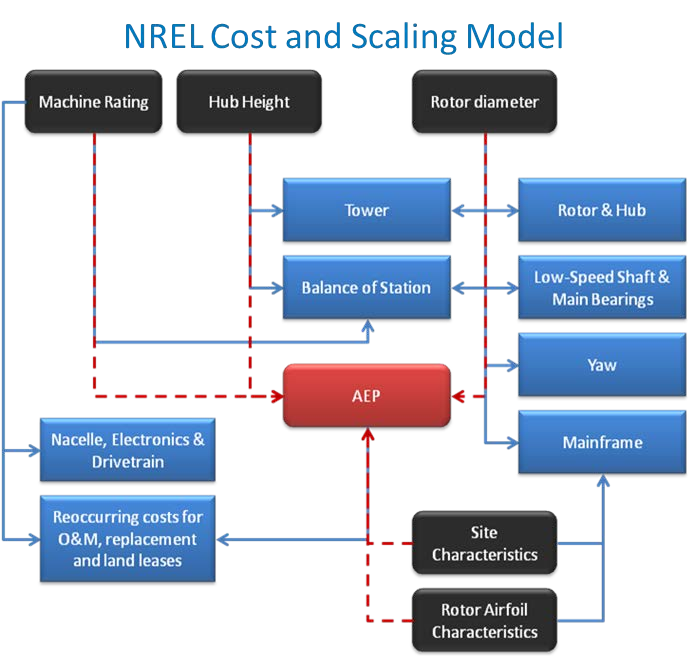
\includegraphics[width=5.5in]{NRELCSM.pdf}
\caption{NREL Cost and Scaling Model Key Input-Output Relationships.}\label{theory:nrelcsm}\end{figure}

The resulting NREL Cost and Scaling Model allows for a variety of interesting analyses including scaling of conventional technology from under a MW to 5 MW+, assessing impact of trends in input factors for materials and labor on wind plant cost of energy, etc.  However, it does not preserve the underlying engineering relationships of the original Sunderland model and thus loses some fidelity of assessing how design changes may impact system costs.

The goal of the development of the following set of models for the hub and nacelle are to return to the mass-based component cost calculations of the original Sunderland Model.  A mass-cost model is developed for each of the major hub and drivetrain component.  These use the NREL Cost and Scaling Model data to estimate relationships that can then be scaled based on economic multipliers as done in {\hyperref[theory:1]{{[}1{]}}}.  Details of the models are described next.


\section{Turbine Component Mass-Cost Models}
\label{theory:turbine-component-mass-cost-models}
A set of models based on the NREL Cost and Scaling model data have been developed to produce relationships of mass-to-cost for all major wind turbine components {\hyperref[theory:1]{{[}1{]}}}.  These in many cases supplant the NREL Cost and Scaling model cost equations for wind turbine components which are often based on a small selection of design parameters such as rotor diameter, hub height and rated power.  The set of wind turbine mass-to-cost models developed include the components: blade, hub system {[}hub, pitch system, and nose cone{]}, nacelle {[}low speed shaft, main bearings, gearbox, high speed shaft/mechanical brake, generator, variable speed electronics, electrical cabling, mainframe {[}bedplate, platforms and railings, base hardware, and crane{]}, HVAC system, controls, and nacelle cover{]}, and tower.  In addition, a mass-to-cost model for offshore monopile foundations has been established based on the new NREL Balance of Station Model {\hyperref[theory:2]{{[}2{]}}}.  This section will describe the mass-to-cost models each of the major wind turbine components.

Blades:
\phantomsection\label{theory:module-twister.models.csm.blades}\index{twister.models.csm.blades (module)}
The new NREL blades mass-cost model is based on the data of the NREL Cost and Scaling Model which was acquired via the WindPACT design studies efforts {\hyperref[theory:3]{{[}3{]}}}.  The data for the blade costs in particular stem from the ``WindPACT Turbine Rotor Design Study'' {\hyperref[theory:4]{{[}4{]}}} as well as the ``Cost Study for Large Wind Turbine Blades:  WindPACT Blade System Design Studies'' {\hyperref[theory:6]{{[}6{]}}}.  The equation for blade costs includes both materials and manufacturing.  The NREL Cost and Scaling Model has built in escalators to update labor and material input cost factors based on cost trends over time.  The model here is reduced to a cost model relationship dependent only on mass as is consistent with the full set of mass-to-cost models.  A graph of the relationships for mass-to-cost from the WindPACT study data based on 2002 USD is shown below.
\begin{figure}[htbp]
\centering
\capstart

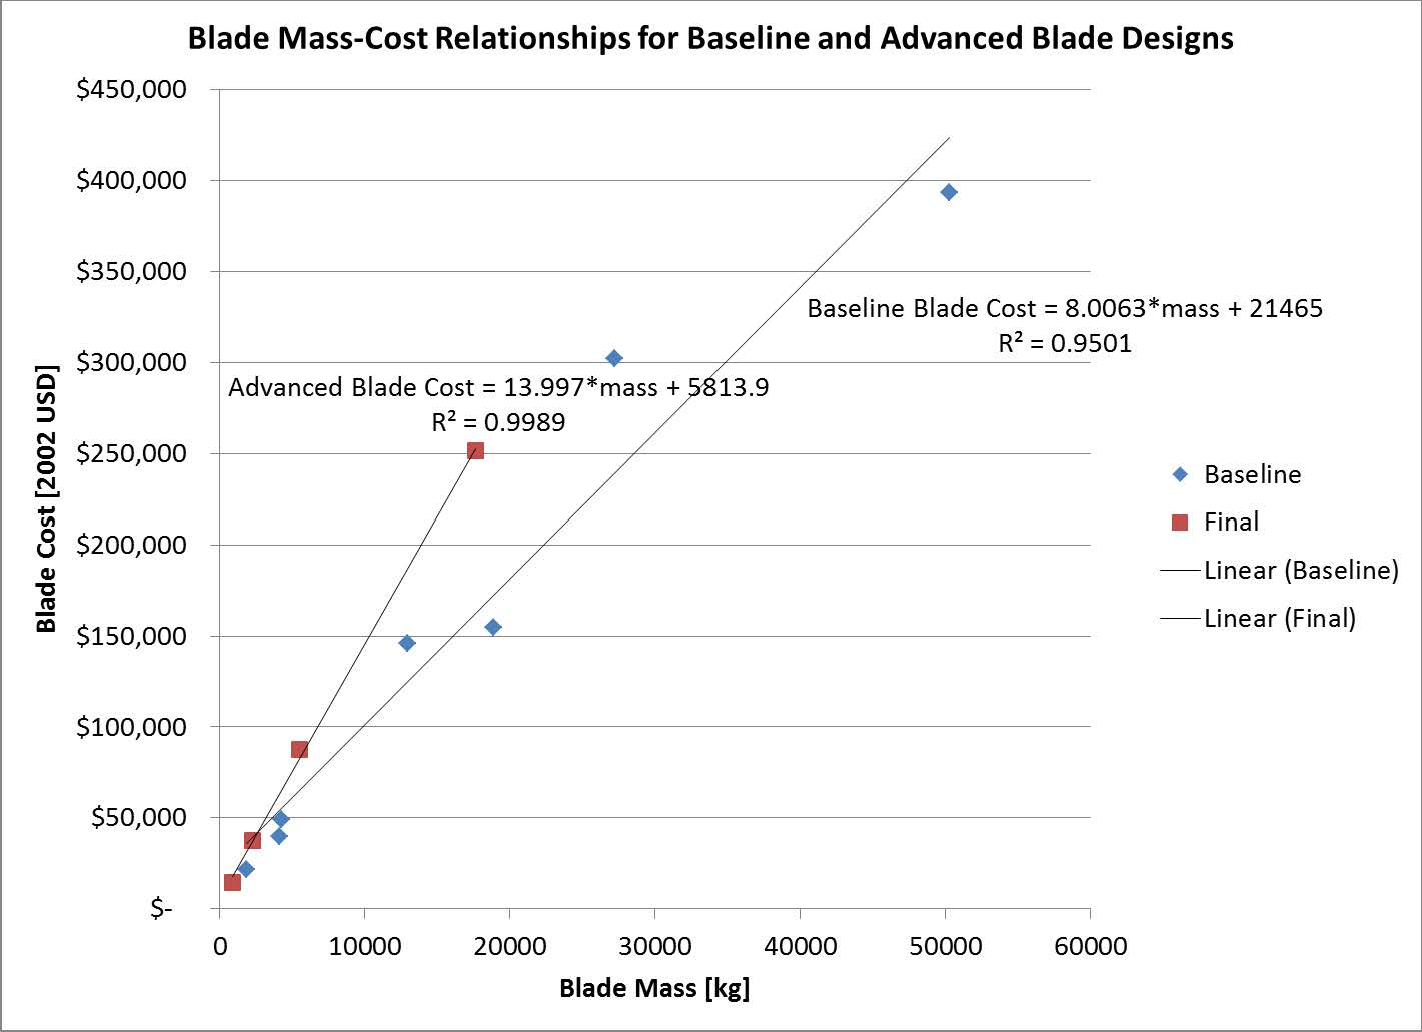
\includegraphics[width=6.5in]{BladeCost.pdf}
\caption{Blade mass-cost relationship based on NREL Cost and Scaling Model.}\label{theory:bladecost}\end{figure}

Hub System:

The cost model for the hub and spinner components are already based on a mass-to-cost relationship and so no adaptation is needed.  For the pitch system, a new mass-to-cost relationship based on the WindPACT study {\hyperref[theory:4]{{[}4{]}}} appendix C for bearing data.  The costs are escalated as described in the NREL Cost and Scaling Model.
\begin{figure}[htbp]
\centering
\capstart

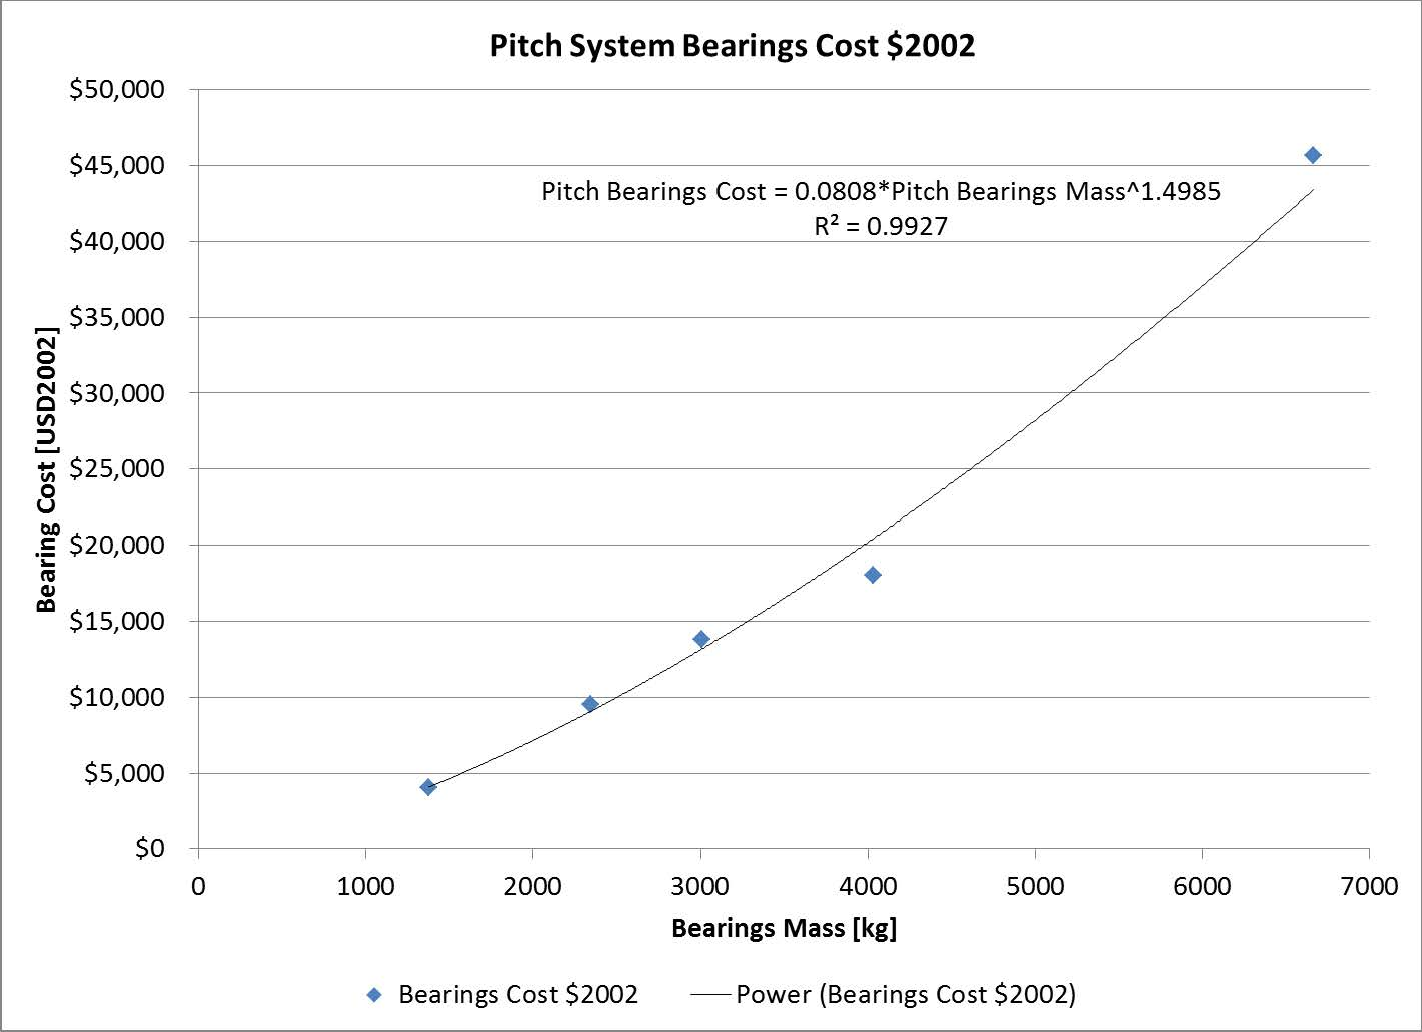
\includegraphics[width=6.5in]{pitchCost.pdf}
\caption{Pitch system mass-cost relationship based on NREL Cost and Scaling Model.}\label{theory:pitchcost}\end{figure}

The mass-cost model for the pitch system was built using the equation as presented on the above figure mutliplied by a factor of 2.28 to account for the pitch system housing as was done in the NREL Cost and Scaling Model.

Drivetrain and Nacelle:

The major components of the low-speed shaft, gearbox, yaw drive and mainframe were adapted to a mass-cost relationship based on data from the WindPACT study {\hyperref[theory:4]{{[}4{]}}}.  The relationship for the main bearings was already mass-based though it had to be divided by a factor of 4 to account for the change in mass estimates from the Sunderland Model.  The relationship for the mechanical brake was an inverse mass-to-cost relationship where the mass was derived by cost by a division of 10 {\hyperref[theory:2]{{[}2{]}}}.  This was adapted to a multiplier of 10 for the mass-cost model.  The generator cost model is as described in {\hyperref[theory:3]{{[}3{]}}} but the costs were updated to the mass-cost relationship of \$65/kg as described in {\hyperref[theory:4]{{[}4{]}}}.  Mass-cost models for rest of the nacelle components could not be made since there is either a lack of data on individual masses and/or costs for such components.  All costs are escalated as described in the NREL Cost and Scaling Model.
\begin{figure}[htbp]
\centering
\capstart

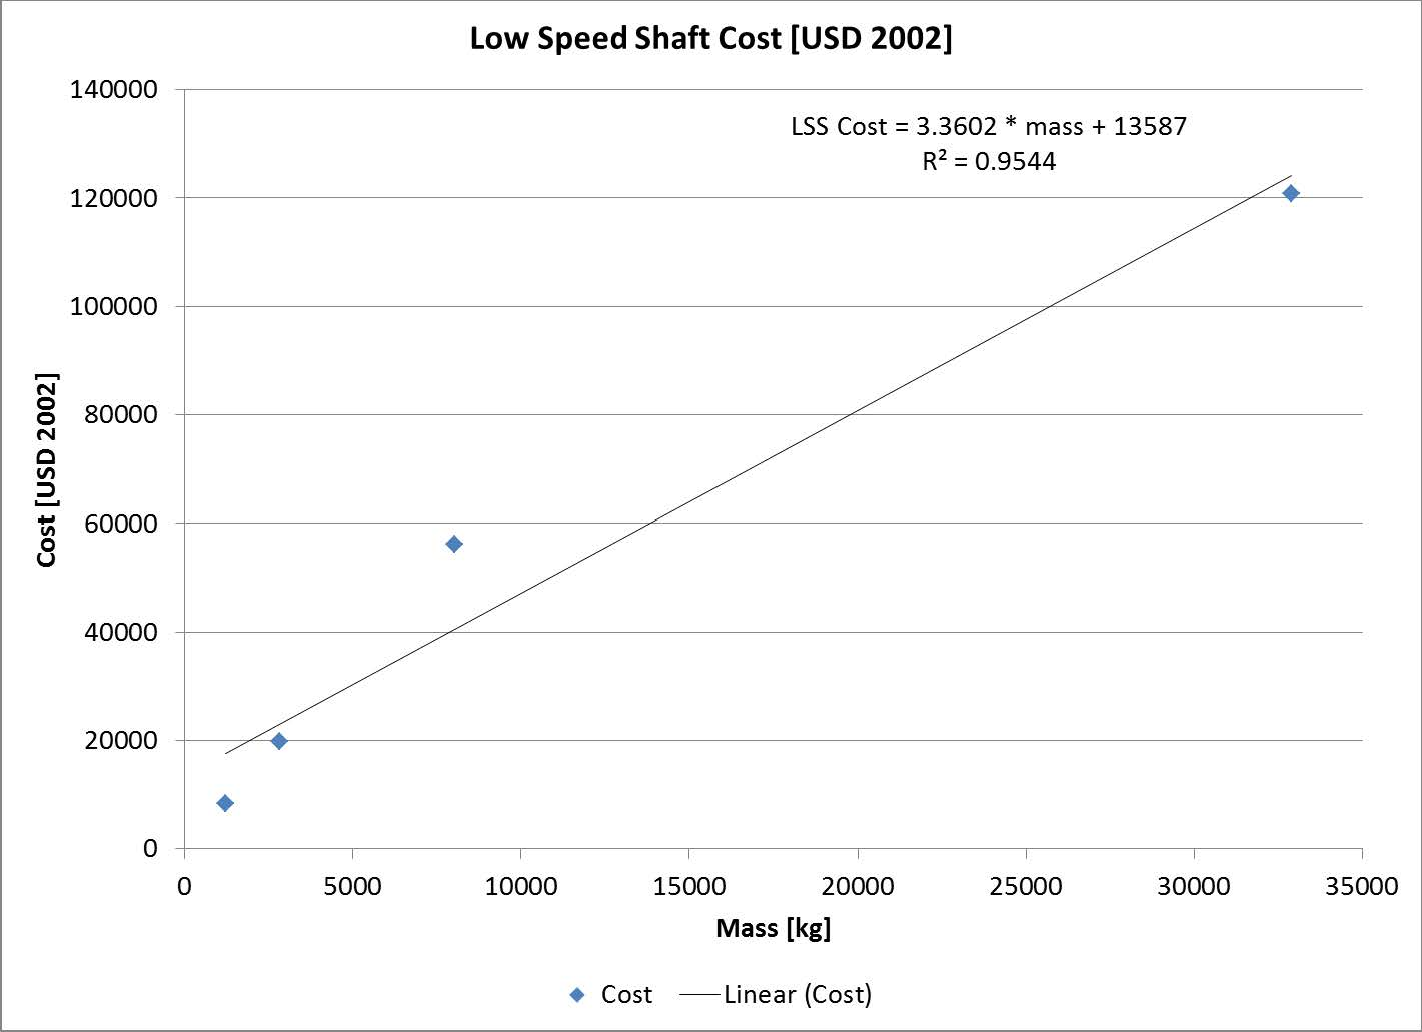
\includegraphics[width=6.5in]{lssCost.pdf}
\caption{LSS mass-cost relationship based on NREL Cost and Scaling Model.}\label{theory:lsscost}\end{figure}
\begin{figure}[htbp]
\centering
\capstart

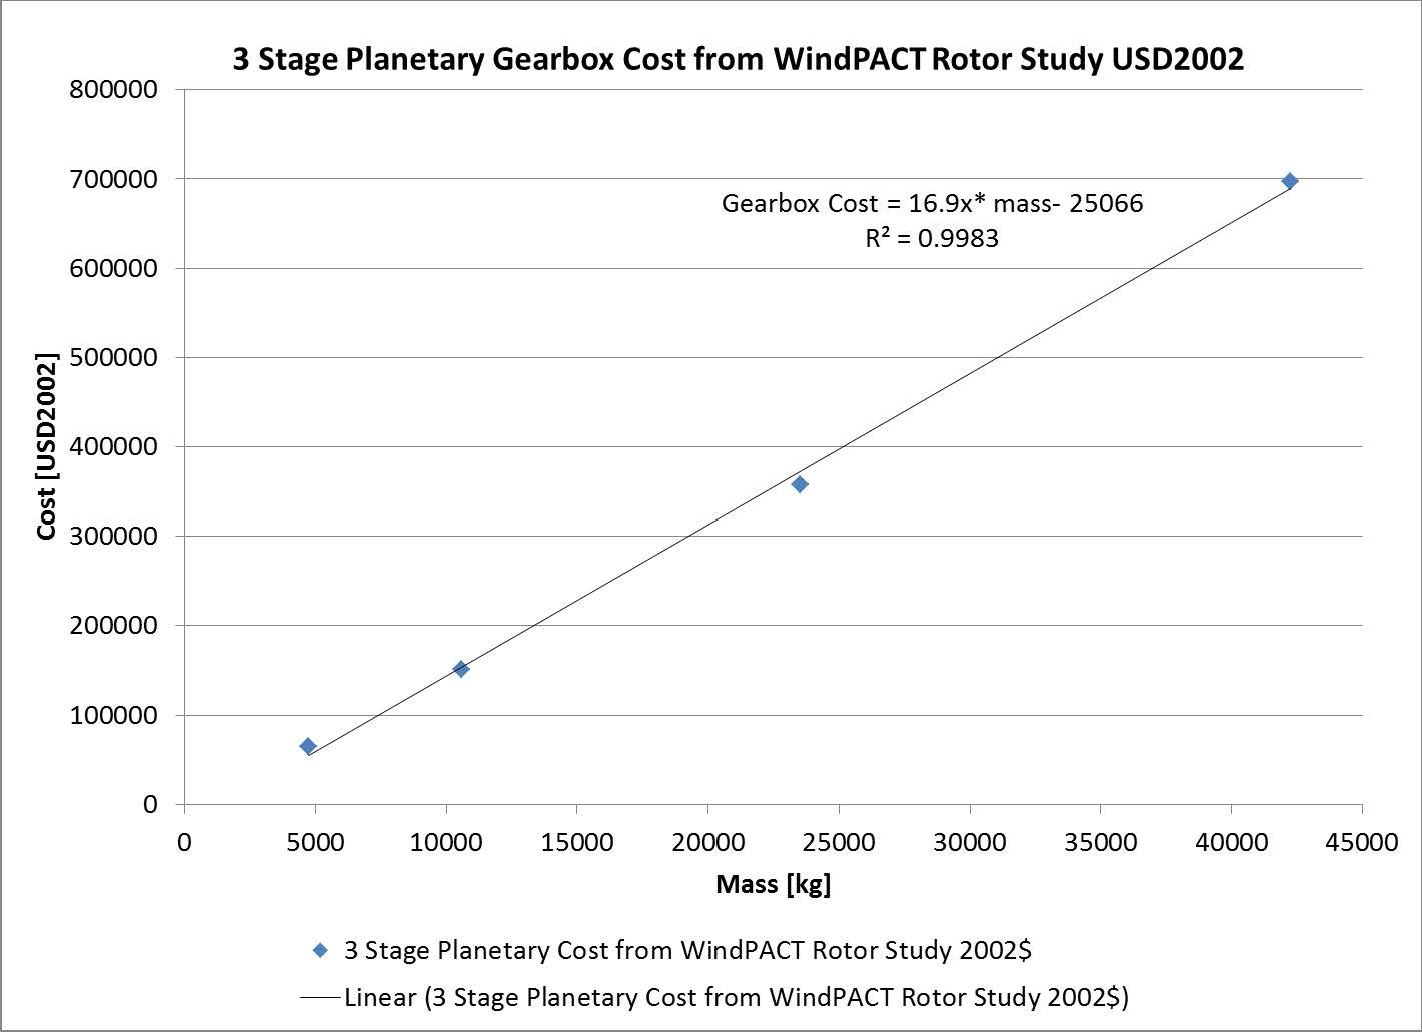
\includegraphics[width=6.5in]{gearboxCost.pdf}
\caption{Gearbox mass-cost relationship based on NREL Cost and Scaling Model.}\label{theory:gearboxcost}\end{figure}
\begin{figure}[htbp]
\centering
\capstart

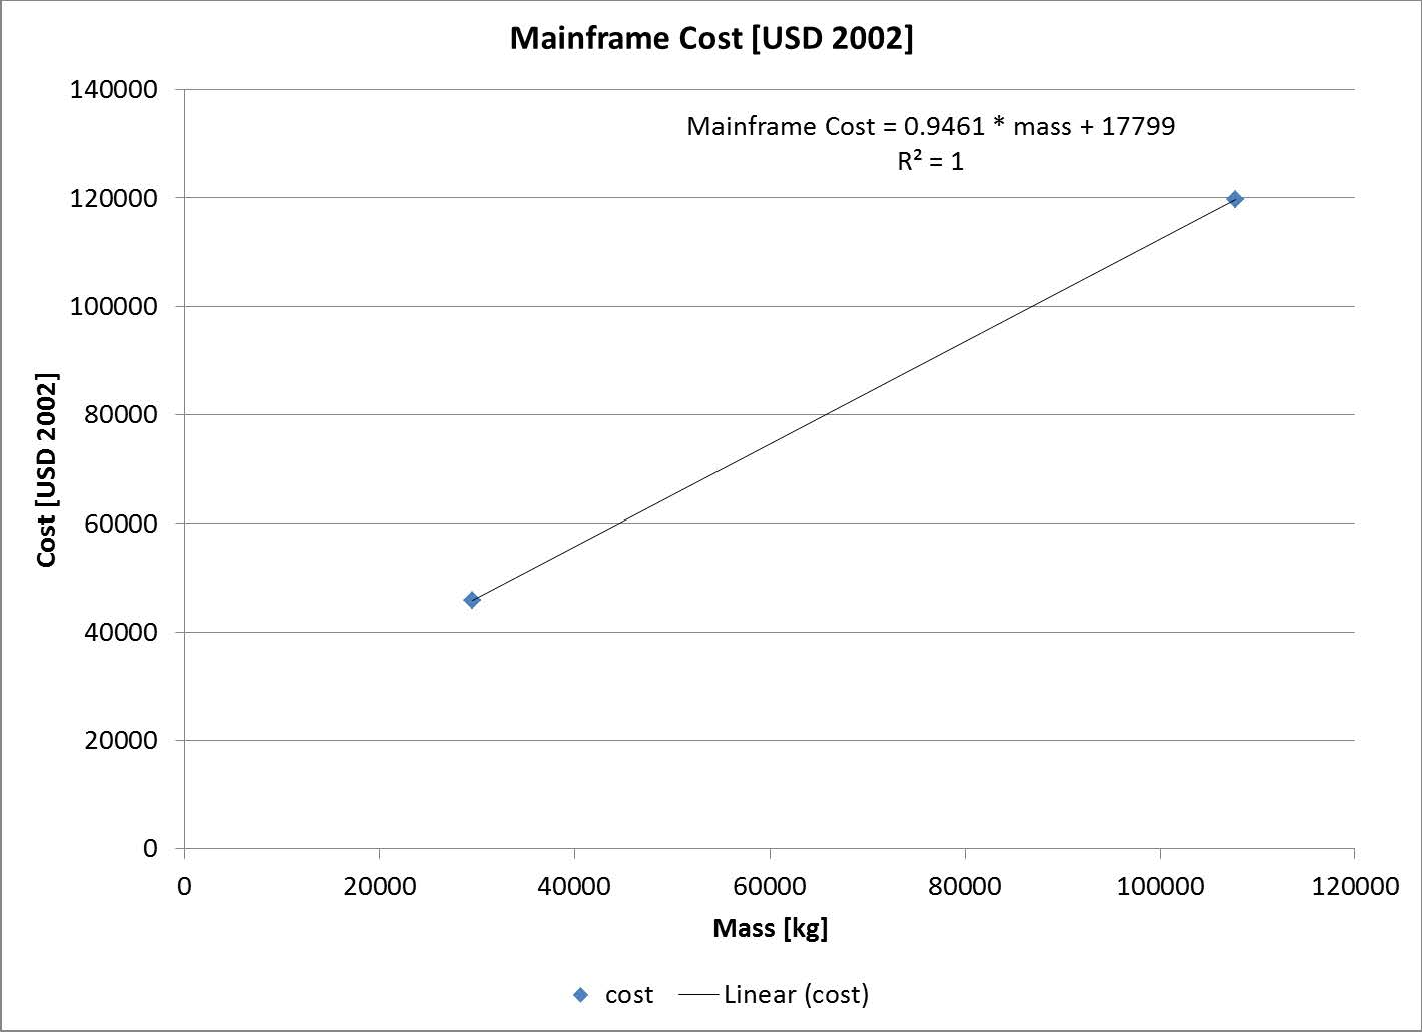
\includegraphics[width=6.5in]{mainframeCost.pdf}
\caption{Mainframe mass-cost relationship based on NREL Cost and Scaling Model.}\label{theory:mainframecost}\end{figure}
\begin{figure}[htbp]
\centering
\capstart

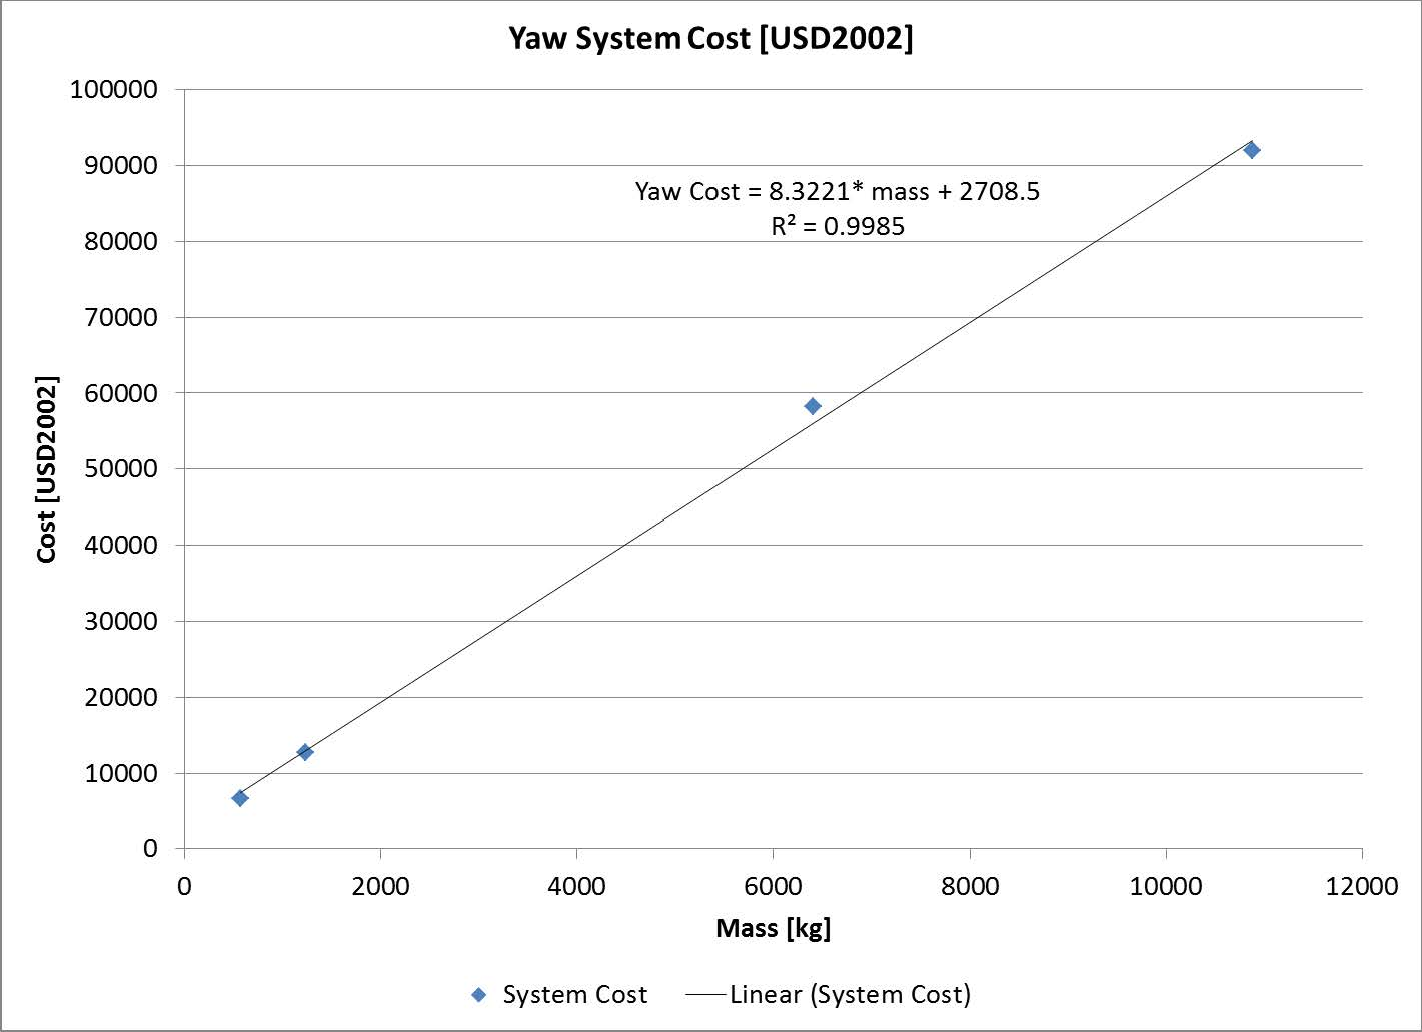
\includegraphics[width=6.5in]{yawCost.pdf}
\caption{Yaw system mass-cost relationship based on NREL Cost and Scaling Model.}\label{theory:yawcost}\end{figure}

The mass-cost models for the components above were built using the equations as presented in the above figures.

Tower:

The NREL tower mass-cost model is identical to the NREL Cost and Scaling Model tower cost model since the model was already based on a mass-to-cost relationship.

Foundation:

The new NREL foundation mass-cost model is based on the new NREL Offshore Balance of Station Model {\hyperref[theory:7]{{[}7{]}}}.  While the model software can be used directly to calculate foundation costs for a variety of offshore configurations, it also calculates the mass of those foundations.  It desirable for a number of analyses to determine the monopile mass directly via an engineering-analysis model.  Thus, this model extracts the foundation cost model (as described in {\hyperref[theory:7]{{[}7{]}}}) so that it can calculate the cost of a monopile foundation directly from the supplied mass of the monopile and transition pieces.  Note that this model is only valid for a monopile type of foundation.  If this model is used in conjunction with the NREL Offshore Balance of Station Model, care must be taken not to double count the foundation cost.



\begin{thebibliography}{1}
\bibitem[1]{1}{\phantomsection\label{theory:1} \DUspan{}{\DUspan{}{\DUspan{}{\DUspan{}{\DUspan{}{\DUspan{}{\DUspan{}{\DUspan{}{L.}\DUspan{}{ }}\DUspan{}{Fingersh}}\DUspan{}{, }\DUspan{}{\DUspan{}{\DUspan{}{M.}\DUspan{}{ }}\DUspan{}{Hand}}}\DUspan{}{, and }\DUspan{}{\DUspan{}{\DUspan{}{A.}\DUspan{}{ }}\DUspan{}{Laxson}}}\DUspan{}{.}}\DUspan{}{ }\DUspan{}{\DUspan{}{Wind turbine design cost and scaling model}\DUspan{}{.}}}\DUspan{}{ }\DUspan{}{\DUspan{}{\DUspan{}{NREL/TP-500-40566}\DUspan{}{, }\DUspan{}{National Renewable Energy Laboratory}\DUspan{}{, }\DUspan{}{Golden, CO}}\DUspan{}{, }\DUspan{}{\DUspan{}{December}\DUspan{}{ }\DUspan{}{2005}}\DUspan{}{.}}}}
\bibitem[2]{2}{\phantomsection\label{theory:2} \DUspan{}{\DUspan{}{\DUspan{}{WindPACT}\DUspan{}{.}}\DUspan{}{ }\DUspan{}{\DUspan{}{Wind partnerships for advanced component technology (windpact)}\DUspan{}{.}}}}
\bibitem[3]{3}{\phantomsection\label{theory:3} \DUspan{}{\DUspan{}{\DUspan{}{\DUspan{}{\DUspan{}{\DUspan{}{\DUspan{}{R.}\DUspan{}{ }}\DUspan{}{Harrison}}\DUspan{}{ and }\DUspan{}{\DUspan{}{\DUspan{}{G.}\DUspan{}{ }}\DUspan{}{Jenkins}}}\DUspan{}{.}}\DUspan{}{ }\DUspan{}{\DUspan{}{Cost modeling of horizontal axis wind turbines}\DUspan{}{.}}}\DUspan{}{ }\DUspan{}{\DUspan{}{\DUspan{}{ETSU/W-34-00170-REP}\DUspan{}{, }\DUspan{}{University of Sunderland, School of Environment}\DUspan{}{, }\DUspan{}{Sunderland, UK}}\DUspan{}{, }\DUspan{}{\DUspan{}{December}\DUspan{}{ }\DUspan{}{1993}}\DUspan{}{.}}}}
\bibitem[4]{4}{\phantomsection\label{theory:4} \DUspan{}{\DUspan{}{\DUspan{}{\DUspan{}{\DUspan{}{\DUspan{}{\DUspan{}{D.J.}\DUspan{}{ }}\DUspan{}{Malcolm}}\DUspan{}{ and }\DUspan{}{\DUspan{}{\DUspan{}{A.C.}\DUspan{}{ }}\DUspan{}{Hansen}}}\DUspan{}{.}}\DUspan{}{ }\DUspan{}{\DUspan{}{Windpact turbine rotor design study}\DUspan{}{.}}}\DUspan{}{ }\DUspan{}{\DUspan{}{\DUspan{}{NREL/SR-500-32495}\DUspan{}{, }\DUspan{}{National Renewable Energy Laboratory}\DUspan{}{, }\DUspan{}{Golden, CO}}\DUspan{}{, }\DUspan{}{\DUspan{}{April}\DUspan{}{ }\DUspan{}{2006}}\DUspan{}{.}}}}
\bibitem[5]{5}{\phantomsection\label{theory:5} \DUspan{}{\DUspan{}{\DUspan{}{\DUspan{}{\DUspan{}{\DUspan{}{\DUspan{}{\DUspan{}{B.}\DUspan{}{ }}\DUspan{}{Maples}}\DUspan{}{, }\DUspan{}{\DUspan{}{\DUspan{}{M.}\DUspan{}{ }}\DUspan{}{Hand}}}\DUspan{}{, and }\DUspan{}{\DUspan{}{\DUspan{}{W.}\DUspan{}{ }}\DUspan{}{Musial}}}\DUspan{}{.}}\DUspan{}{ }\DUspan{}{\DUspan{}{Comparative assessment of direct drive high temperature superconducting generators in multi-megawatt class wind turbines}\DUspan{}{.}}}\DUspan{}{ }\DUspan{}{\DUspan{}{\DUspan{}{NREL/TP-5000-49086}\DUspan{}{, }\DUspan{}{National Renewable Energy Laboratory}\DUspan{}{, }\DUspan{}{Golden, CO}}\DUspan{}{, }\DUspan{}{\DUspan{}{October}\DUspan{}{ }\DUspan{}{2010}}\DUspan{}{.}}}}
\bibitem[6]{6}{\phantomsection\label{theory:6} \DUspan{}{\DUspan{}{\DUspan{}{\DUspan{}{\DUspan{}{\DUspan{}{TPI}\DUspan{}{ }\DUspan{}{Composites}}\DUspan{}{ }}\DUspan{}{Inc.}}\DUspan{}{ }\DUspan{}{\DUspan{}{Cost study for large wind turbine blades: windpact blade system design studies}\DUspan{}{.}}}\DUspan{}{ }\DUspan{}{\DUspan{}{\DUspan{}{SAND/2003-1428}\DUspan{}{, }\DUspan{}{Sandia National Laboratories}\DUspan{}{, }\DUspan{}{Albuquerque, NM}}\DUspan{}{, }\DUspan{}{\DUspan{}{May}\DUspan{}{ }\DUspan{}{2003}}\DUspan{}{.}}}}
\bibitem[7]{7}{\phantomsection\label{theory:7} \DUspan{}{\DUspan{}{\DUspan{}{\DUspan{}{\DUspan{}{\DUspan{}{B.}\DUspan{}{ }}\DUspan{}{Maples}}\DUspan{}{.}}\DUspan{}{ }\DUspan{}{\DUspan{}{Offshore balance of station model - forthcoming}\DUspan{}{.}}}\DUspan{}{ }\DUspan{}{\DUspan{}{\DUspan{}{NREL/TP-5000-xxxxxx}\DUspan{}{, }\DUspan{}{National Renewable Energy Laboratory}\DUspan{}{, }\DUspan{}{Golden, CO}}\DUspan{}{, }\DUspan{}{\DUspan{}{TBD}\DUspan{}{ }\DUspan{}{TBD}}\DUspan{}{.}}}}
\end{thebibliography}



\end{document}
